\section{Evaluation}
\label{sec:eval}

Our evaluation asks three questions. Does accounting beat the two baselines that a
practitioner would use instead (\S\ref{sec:eval-main})? Where does the time go---is the win
an admission effect or a cache effect (\S\ref{sec:eval-decomp})? And when does it stop
paying (\S\ref{sec:eval-neg})? We fix the metrics and the decision criteria before running,
and report every arm on every metric whether or not it favours the design.

\subsection{Setup and metrics}
\label{sec:eval-setup}

All arms replay the same 19-session, 602-round trace on the same GPU, model, memory
fraction, and cache configuration (\S\ref{sec:impl}); they differ only in the controller.
We report five quantities, defined once and computed by one script from the per-step logs.

\emph{Makespan}: the time from the first arrival to the last completion---the batch time a
server operator cares about. \emph{Session end-to-end}: for each session, the time from its
arrival to its own last completion; we report the median and the 90th percentile, because
the mean hides the tail. \emph{Round latency}: for each round, the time from the moment the
session \emph{could} continue (its arrival, or the end of the previous round plus the
simulated tool wait) to the first output token. This is the quantity a user experiences,
and it includes both the time the controller makes the session wait at the door and the
time the engine takes to produce a token; reporting engine-side TTFT alone would hide
exactly the cost that admission control imposes. \emph{Deadline miss rate}: the fraction of
rounds whose round latency exceeds 10\,s, the per-round budget we fixed in advance.
\emph{Goodput}: rounds that meet the deadline per hour of makespan, which normalises for
the fact that a faster batch also has less wall time in which to accumulate hits.
\emph{Work}: the sum of uncached prompt tokens and completion tokens, i.e.\ the prefill the
engine actually had to do, which is the quantity the mechanism claims to reduce.

\subsection{Main result}
\label{sec:eval-main}

Table~\ref{tab:main} reports the three arms.

\begin{table*}[t]
\caption{Three arms, same trace, engine, and memory budget. Round latency includes the
controller's door wait and the engine's TTFT; the deadline is 10\,s per round. Work is
uncached prefill plus completion tokens.}
\label{tab:main}
\centering
\small
\begin{tabular}{@{}lccc@{}}
\toprule
 & request-level & agent-level & \sys{} \\
\midrule
makespan (min) & \pend{ms-A} & \pend{ms-B} & 154.9 \\
session end-to-end, median (min) & \pend{e2e-A} & \pend{e2e-B} & 115.6 \\
session end-to-end, p90 (min) & \pend{e2e90-A} & \pend{e2e90-B} & 151.8 \\
round latency, median (s) & \pend{r50-A} & \pend{r50-B} & 9.7 \\
round latency, p90 (s) & \pend{r90-A} & \pend{r90-B} & 291.9 \\
rounds missing 10\,s (\%) & \pend{miss-A} & \pend{miss-B} & 49.8 \\
goodput (rounds/h) & \pend{gp-A} & \pend{gp-B} & 105.4 \\
work (Mtok) & \pend{work-A} & \pend{work-B} & 9.00 \\
KV reuse (\%) & \pend{hit-A} & \pend{hit-B} & 65.2 \\
\bottomrule
\end{tabular}
\end{table*}

The capacity-accounted arm finishes the 542 rounds it completed in 154.9 minutes. Its
engine was busy for 67.8\% of the wall clock and idle for 51.1 minutes; it served 65.2\%
of its prompt tokens from cache---43.7\% from the device tier and 21.5\% from the host
tier---and still re-read 4.43 times the tokens it appended, evicting 15.3M tokens to do
so. The median round returns in 9.7\,s, but the tail does not: the 90th percentile is
291.9\,s, and half of the rounds miss the 10\,s budget. \pend{comparison against the two
baselines on the common completion set, and which of the four pre-registered criteria
hold.}

\subsection{Where the time goes}
\label{sec:eval-decomp}

A faster makespan can come from three places: the engine does less work (fewer uncached
prefill tokens), the engine is busier (less idle time while sessions are parked), or the
work is better overlapped. We separate them from the logs, without running anything new.
The re-read tax is the ratio of uncached prefill to appended tokens: it is $1$ when every
session's prefix is retained and grows when state is lost.

\begin{table*}[t]
\caption{Decomposition. Busy and idle time are sampled from the engine's running-request
count over each run's window. Prompt, device-hit and host-hit tokens are the engine's
cumulative counters over the same window; uncached prefill, completion and the re-read tax
are summed from the per-step records. Evicted tokens are what the engine had to throw away
to make room.}
\label{tab:decomp}
\centering
\small
\begin{tabular}{@{}lccc@{}}
\toprule
 & request-level & agent-level & \sys{} \\
\midrule
busy time (min) & \pend{busy-A} & \pend{busy-B} & 107.5 \\
idle time (min) & \pend{idle-A} & \pend{idle-B} & 51.1 \\
prompt tokens (Mtok) & \pend{pr-A} & \pend{pr-B} & 25.23 \\
uncached prefill (Mtok) & \pend{unc-A} & \pend{unc-B} & 8.77 \\
completion (Mtok) & \pend{dec-A} & \pend{dec-B} & 0.23 \\
device hits (\%) & \pend{dh-A} & \pend{dh-B} & 43.7 \\
host hits (\%) & \pend{hh-A} & \pend{hh-B} & 21.5 \\
evicted tokens (Mtok) & \pend{ev-A} & \pend{ev-B} & 15.32 \\
re-read tax ($\times$ append) & \pend{rr-A} & \pend{rr-B} & 4.43 \\
\bottomrule
\end{tabular}
\end{table*}

\pend{paragraph interpreting the decomposition, including the cases where the design wins on
work but not on busy time, or vice versa.}

\subsection{Where the recompute comes from}
\label{sec:eval-attrib}

Table~\ref{tab:decomp} says how much work was redone; it does not say who caused it. We
classify every round of an arm by what happened between the previous round's completion and
this round's submission: the round is the session's \emph{first} (nothing to reuse), it
followed a \emph{suspension} by the controller, or it was \emph{continuous} (admitted
throughout, so a miss is the engine's own eviction). The classification is mechanical---it
reads the admission event log and the step log, and needs no new run.

\begin{table}[t]
\caption{Attribution of the re-read tax in the capacity-accounted arm. Rounds are classified
by what happened between the previous round and this one. \emph{rounds} and \emph{share} are
percentages, \emph{uncached} is in millions of tokens, and \emph{excess} is uncached prefill
divided by the tokens the round actually appended.}
\label{tab:attrib}
\centering
\footnotesize
\begin{tabular}{@{}lccc@{}}
\toprule
 & first & susp. & cont. \\
\midrule
rounds & 3.5 & 24.9 & 71.6 \\
uncached (M) & 0.33 & 4.80 & 3.65 \\
share & 3.7 & 54.7 & 41.6 \\
excess & 1.75 & 6.99 & 3.29 \\
\bottomrule
\end{tabular}
\end{table}

Table~\ref{tab:attrib} gives the answer for the capacity-accounted arm. Of its 8.77M
uncached prefill tokens, 3.7\% are first rounds that no policy can avoid, 41.6\% belong to
rounds that were never suspended---the engine evicted the prefix on its own---and
\emph{54.7\% follow a suspension by our own controller}. In those rounds the excess is
$7.0\times$ the tokens the round actually appended and 68\% are full recomputations:
suspension is the largest single source of recompute in our own arm.

The same decision is what keeps the engine fed. Over the 138 suspensions of the run
(20.4 hours of session-time in total), the engine was running another session's round in
72.1\% of the sampled intervals. The host tier holds only a few sessions---203K tokens
against a 1.31M working set---so most suspensions cannot keep the state they suspend; the
ledger is choosing which state to lose, and it is paying for that choice with the
recompute in Table~\ref{tab:attrib}. This is the empirical form of the claim that the
slot, not the copy, is the scarce resource, and it is the cost that the two baselines are
compared against in \S\ref{sec:eval-main}.

\subsection{Mechanism, in one session}
\label{sec:eval-timeline}

\begin{figure}[t]
\centering
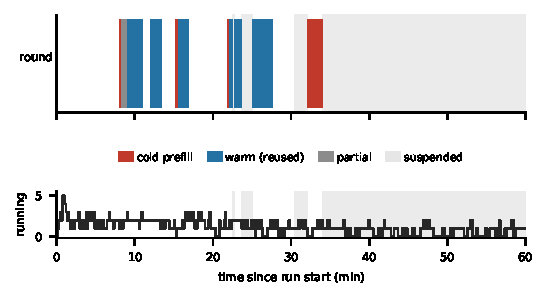
\includegraphics[width=\columnwidth]{figs/fig_timeline.pdf}
\caption{One session of the capacity-accounted arm (39 rounds, 17 suspensions), first hour.
Each bar is a round, coloured by how much of its prefix the engine had to recompute; grey
spans are suspensions. The lower panel is the engine's running-request count: while the
session is suspended the card keeps serving other sessions, which is the slot the
suspension buys. A round that follows a suspension is usually red---the state did not
survive---which is the cost side of the same decision.}
\label{fig:timeline}
\end{figure}

\pend{paragraph reading the timeline: how often the session was suspended, what the
suspension cost (revival vs recompute counts), and whether the slot was picked up by
another session while it was parked.}

\subsection{Log-based counterfactual: concurrency or state?}
\label{sec:eval-cf}

Our design differs from the agent-level baseline in two ways at once: it accounts for
capacity, and it preserves state. To separate the two without another run, we replay the
controller's own decisions offline and ask what would have happened under a concurrency-only
variant of the same controller---same permits, same pausing, but no host-tier accounting
and no revival pricing.

\pend{the counterfactual numbers and the sentence that says how much of the gain comes from
each half.}

\subsection{When it does not pay}
\label{sec:eval-neg}

We report three regimes in which the mechanism loses or is neutral, and we say why.
\emph{(i) Ample capacity.} If the working set fits, nothing is suspended, the ledger reduces
to first-come-first-served, and the only difference from the request-level arm is a small
amount of bookkeeping; the design cannot win and does not claim to. \emph{(ii) Short
contexts.} If a round's context is small, the recompute is cheap and the break-even
\eqref{eq:ratio} favours recomputation; suspension then buys nothing. \emph{(iii) Saturated
engine.} When the engine is already busy, adding admission discipline removes capacity from
the queue and can increase the tail, because the door wait moves from a place where it
overlaps with other work to a place where it does not.

\pend{the measured instances of (i)--(iii) in the arms, and the sensitivity to $\rho$ and
$t^\ast$.}

\subsection{Threats to validity}
\label{sec:eval-threats}

Every arm is a single run of one trace on one GPU, so we report measured differences and
full distributions rather than significance tests; run-to-run variation is visible only in
the per-session scatter, and a single batch cannot separate policy effects from the
particular interleaving. The trace is reconstructed from agent transcripts rather than
observed in production, and all sessions arrive together, which is the worst case for
admission and the best case for a batch controller. The model is a 7B coding model on a
24\,GB card; the constants in \S\ref{sec:analysis} would differ on other hardware, though
the quantities in which the argument is stated would not.
